\documentclass[../main.tex]{subfiles}

\begin{document}

\chapter{Design}
\section{Overview}

\section{Data synthesis}
Studies in human cognition by \textcite{bilalic2010} and \textcite{zhou2018} compared skilled chess players with novices in terms of their ability to remember a chess position for a short amount time confirmed that highly skilled players outperform novices at this task.
Perhaps more interestingly, both studies found that skilled players remembered \emph{random} positions (where pieces are positioned on random squares, not necessarily obeying the rules of chess) significantly less accurately than they did positions from actual chess games. 
Thus it stands to reason that in general, highly skilled chess players exhibit a more developed pattern recognition ability for chess positions than novices, but this ability is specific to positions that conform to the rules of chess and are likely to occur in actual games.

This project aims to develop a similar pattern recognition ability using machine learning, and therefore our dataset will consist of positions from real chess games. 
In doing so, we automatically ensure that the chess positions are legal according to chess rules such that a probabilistic reasoning system could later yield sensible results in a post-processing step (see Objective 2.2).

\subsection{Chess positions}
The positions are generated from a publicly available dataset of 2,851 games played by current World Chess Champion Magnus Carlsen \cite{64squares2020}.
Each move in each game is included in our dataset with a probability of 2\%, and duplicate positions are discarded.
A total of 4,888 chess positions are obtained in this manner and saved in \gls{fen} format.

\subsection{Three-dimensional renders}
In order to obtain realistic images of these chess positions, we employ a three-dimensional model of a chess set on a wooden table. 
Chess pieces are placed on the board squares according the given \gls{fen} description. 
Different camera angles and lighting setups are chosen in a random process in order to maximise diversity in the dataset.

\begin{figure}
    \centering
    \begin{tikzpicture}
        \begin{axis}[
            axis lines=middle,
            xlabel=$x$,
            ylabel=$y$,
            x=.75cm, y=.75cm,
            xmin=-4, xmax=4,
            ymin=-4, ymax=4,
            enlargelimits,
            clip=false
        ]
            \foreach \y in {-4,-2,...,2}{
                \foreach \x in {-4,-2,...,2}{
                    \edef\temp{\noexpand\fill[pattern=crosshatch, pattern color=black] (\x,\y) rectangle (1+\x,1+\y) rectangle (2+\x,2+\y);}
                    \temp
                };
            };
            \draw (-4, -4) rectangle (4, 4);
            \draw[->] (6, -1) -- (6, 1) node[above,align=center] {direction of play \\ (white)};
        \end{axis}
    \end{tikzpicture}
    \caption[The chessboard coordinate system.]{Overhead view of the coordinate system on the chessboard. The $z$-axis (not shown) points upward, normal to the chessboard surface, and the board is oriented like a chess game would be set up, i.e. the bottom right square is white. White's direction of play (the direction in which pawns are advanced) coincides with the $y$-axis.}
    \label{fig:cartesian_chessboard}
\end{figure}
Let us consider a three-dimensional Cartesian coordinate system whose origin lies at the centre point of the chessboard's surface, as depicted in \cref{fig:cartesian_chessboard}. 
The chessboard lies on the plane formed by the $x$ and $y$ axes, and the chess squares are of unit length. 

\paragraph{Pieces}
The pieces are positioned on the squares as dictated by the particular \gls{fen} description.
However, instead of positioning them at the centre in their respective squares, they are randomly rotated and positioned with a random offset to emulate the conditions in real chess games.
More specifically, the $x$ and $y$ position of a piece in file $i$ and rank $j$ is sampled from a bivariate normal distribution given by
\(
    \rvp_{i,j} \sim \normal \left(
        \begin{bmatrix}
            i \\ j
        \end{bmatrix} - \frac{7}{2},
        \frac{\mI_2}{10}
    \right).
\)
Here, we assume that $i$ and $j$ are zero-indexed, i.e. the square \emph{a1} corresponds to $i=j=0$.
The reason for shifting the mean by $\frac{7}{2}$ above is that since the origin lies at the midpoint of the board, the mean must be shifted four units to the left (or downwards for the $y$-axis), but since the normal distribution should be centred on the midpoint of the square, we must add one half.
Due to the fact that the $x$ and $y$ axes are perpendicular, the two components of $\rvp$ will be independent and thus can be modelled with a covariance matrix that is a multiple of the identity matrix $\mI_2$.
Experiments showed that a variance of $\frac{1}{10}$ achieved realistic results.
Finally, the piece's rotation about its $z$-axis is sampled from a uniform distribution over the half-open interval $[0, 2\pi)$.

\paragraph{Camera}
The camera is aligned such that it points directly at the origin (i.e. the centre of the board).
It is positioned with only a small offset from the $yz$-plane to ensure that the view over the chessboard is similar to the current player's perspective. 
A slight perturbation to the $x$-component of the camera position is introduced according to a normal distribution with $\mu=0$ and $\sigma=0.8$ since the player will not usually be positioned exactly in the middle in front of the board.
An angle $\theta$ is chosen uniformly in the range $\left[\frac{\pi}{4},\frac{\pi}{3}\right]$ to represent the angle that the camera makes with the board's surface (see \cref{fig:camera_angle}) if white is to play%
\footnote{On the other hand, if it is black to play, the perspective must be from the other side of the board, so $\theta$ is chosen in the range $\left[\frac{2\pi}{3},\frac{3\pi}{4}\right]$ which is equivalent to reflecting the camera position about the $xz$-plane.}.
\begin{figure}
    \centering
    \begin{tikzpicture}
        \begin{axis}[
            % axis lines=middle,
            xlabel=$y$,
            ylabel=$z$,
            x=.5cm, y=.5cm,
            xmin=-7, xmax=7,
            ymin=0, ymax=8,
            enlargelimits
        ]
            \coordinate (cam) at (7, 7);
            \coordinate (center) at (0, 0);
            \coordinate (end) at (4, 0);
            \draw[|-|] (-4, 0) -- (4, 0) node[near start,fill=white] {board};
            \draw[->,dashed] (cam) -- (0, 0);
            \draw (cam) -- (6, 6.7) -- (6.7, 6) -- (cam) node[above] {camera};
            \pic[draw, ->, "$\theta$", angle radius=1cm] {angle = end--center--cam};
        \end{axis}
    \end{tikzpicture}
    \caption{Side view of the camera setup for the scenario where it is white to move. }
    \label{fig:camera_angle}
\end{figure}
This range is chosen because human players would typically choose a camera angle between 45 and 60 degrees to ensure maximum visibility of the pieces.
The two remaining components ($y$ and $z$) of the camera's location is then obtained using a simple trigonometric calculation such that the distance from the camera to the origin is $11$ units, a length that allows the camera to capture the entire board.

\paragraph{Lighting}
For each chess position, a random choice is made between two different lighting scenarios, each having equal probability of being employed.
\begin{enumerate}
    \item The first lighting mode tries to emulate a \emph{camera flash}.
        To do so, a spotlight is set up with the same location and orientation as the camera. 
        As a result, the scene is light up quite well with no large shadows, as it can be seen in \cref{fig:lighting_flash_example}.
        \begin{figure}
            \centering
            \begin{subfigure}[b]{0.47\textwidth}
                \centering
                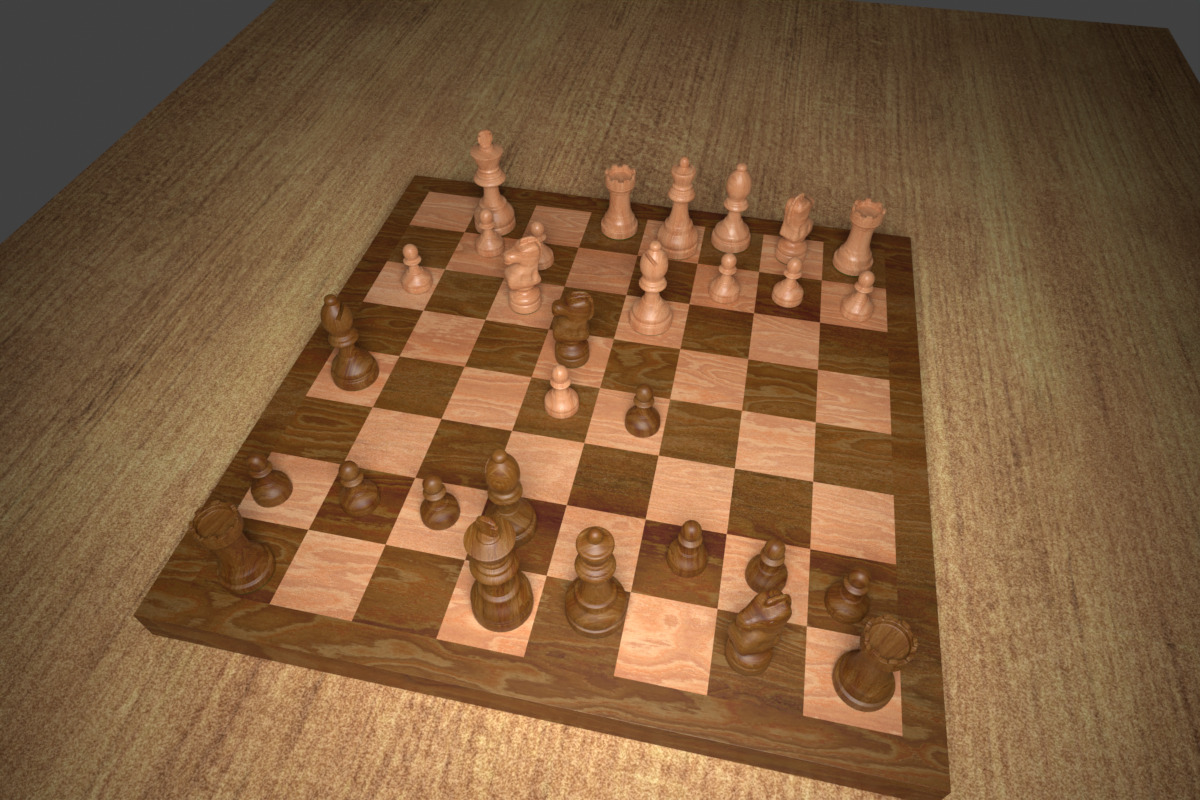
\includegraphics[width=\textwidth]{lighting_flash}
                \caption{camera flash}
                \label{fig:lighting_flash_example}
            \end{subfigure}
            \hfill
            \begin{subfigure}[b]{0.47\textwidth}
                \centering
                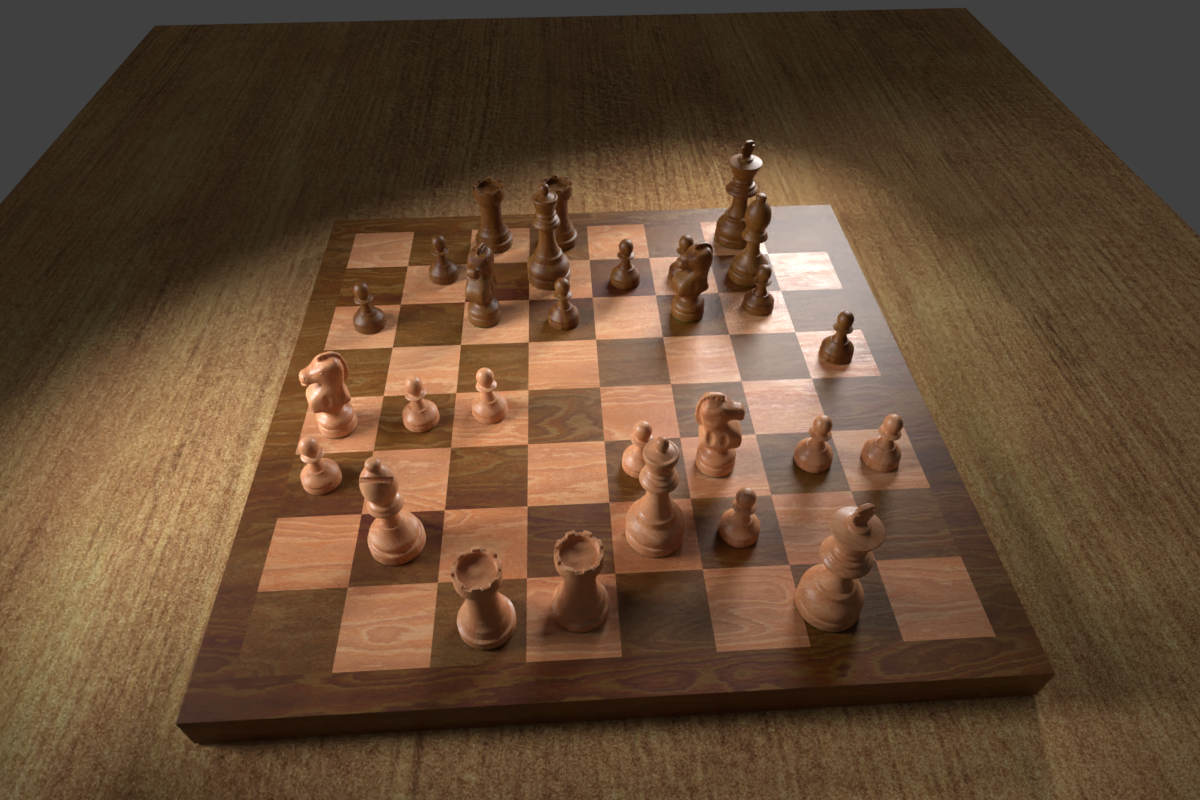
\includegraphics[width=\textwidth]{lighting_spotlights}
                \caption{spotlights}
                \label{fig:lighting_spotlights_example}
            \end{subfigure}
            \caption{Two samples from the synthesised dataset showing both types of lighting.}
            \label{fig:lighting_examples}
        \end{figure}
    \item In the other lighting mode, two spotlights are set up in the scene. 
        Their $x$ and $y$ coordinates are constrained such that they lie on a circle centred at the origin of the coordinate system with radius 10 on the $xy$-plane, as depicted in \cref{fig:chessboard_lighting_circle}, but each spotlight's location along the circumference is sampled uniformly.
        \begin{figure}
            \centering
            \begin{tikzpicture}
                \begin{axis}[
                    axis lines=middle,
                    xlabel=$x$,
                    ylabel=$y$,
                    x=.4cm, y=.4cm,
                    xmin=-10, xmax=10,
                    ymin=-10, ymax=10,
                    enlargelimits,
                    clip=false
                ]
                    \foreach \y in {-4,-2,...,2}{
                        \foreach \x in {-4,-2,...,2}{
                            \edef\temp{\noexpand\fill[pattern=crosshatch, pattern color=black] (\x,\y) rectangle (1+\x,1+\y) rectangle (2+\x,2+\y);}
                            \temp
                        };
                    };
                    \draw (-4, -4) rectangle (4, 4);

                    
                    \coordinate (o) at (0, 0);
                    \coordinate (s1) at (45:10);
                    \coordinate (s2) at (135:10);
                    \draw[dashed] (o) circle (10);
                    \draw[dashed,->] (s1) -- (o);
                    \draw[dashed,->] (s2) -- (o);

                    \draw (s1) -- (5.3, 6.3) -- (6.3, 5.3) -- cycle node[right] {spotlight 1};
                    \draw (s2) -- (-5.3, 6.3) -- (-6.3, 5.3) -- cycle node[left] {spotlight 2};
                \end{axis}
            \end{tikzpicture}
            \caption{Overhead view of the chessboard with two spotlights. The spotlights are constrained to the dashed circle such that their distance to the origin amounts to 10 units when disregarding the $z$-component.}
            \label{fig:chessboard_lighting_circle}
        \end{figure}
        Furthermore, each spotlight's $z$-component is sampled uniformly in the range $[5, 10)$.
        Finally, the for each spotlight, a focus point on the chessboard surface (i.e. the $xy$ plane) is sampled from
        \(
            \normal\left(
                \begin{bmatrix}
                    0 \\ 0
                \end{bmatrix},
                \frac{5}{2} \mI_2
            \right)
        \)
        and the corresponding spotlight is rotated such that it points in that direction.
        Consequently, there is greater variabililty in the lighting because the spotlights could be pointing at different areas of the board, thus producing different types of shadows.
        \Cref{fig:lighting_spotlights_example} shows an example rendering where the lighting produced by the spotlights is poorer than the camera flash mode.
\end{enumerate}

\subsection{Automated labelling}
\todo{use the chesscog.data\_synthesis.visualisation script}
\todo{todo: explain how dataset was split into train/val/test}

\section{A classification-based approach}
\subsection{Board detection}
\todo{TODO: corner point detection}
\subsection{Occupancy classification}
\label{sec:occupancy_classification}

Empirical experiments showed that performing piece classification directly after detecting the four corner points with no intermediate step yields a large number of false positives, i.e. empty squares being classified as containing a chess piece.
\begin{figure}
    \centering
    \begin{subfigure}[b]{0.65\textwidth}
        \centering
        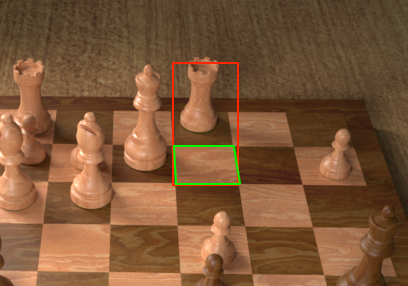
\includegraphics[width=\textwidth]{3828_annotated}
        \caption{region from the original image with marked square}
        \label{fig:occupancy_classification_fp_original}
    \end{subfigure}
    \hfill
    \begin{subfigure}[b]{0.3\textwidth}
        \centering
        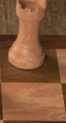
\includegraphics[width=.7\textwidth]{3828_cut}
        \caption{cropped sample}
        \label{fig:occupancy_classification_fp_cropped}
    \end{subfigure}
    \caption[An example illustraing why an immediate piece classification approach is inclined to reporting false positives.]{An example illustraing why an immediate piece classification approach is inclined to reporting false positives. Consider the square marked in green in the original image \subref{fig:occupancy_classification_fp_original}. The bounding box for piece classification (marked in red) must be quite tall because the square might contain a tall piece such as a queen or king (the box must be at least as tall as the the queen in the adjacent square on the left). The resulting sample, depicted in \subref{fig:occupancy_classification_fp_cropped}, contains almost the entire rook of the square behind. Thus, a piece classifier might classify this square as containing a rook instead of being empty.}
    \label{fig:occupancy_classification_fp}
\end{figure}
One common scenario where the trained classifier failed is illustrated in \cref{fig:occupancy_classification_fp}.
Notice that squares further away from the camera must be cropped with increasingly taller bounding boxes.
If a particular square is empty but its bounding box includes the piece from the adjacent square as in \cref{fig:occupancy_classification_fp_cropped}, the trained classifier was inclined to report a false positive.

To solve this problem, a binary classifier is trained on cropped squares to decide whether they are empty or not.
Before cutting out the squares from the original image, the input image is warped to a two-dimensional overhead view by means of a projective transformation.
This ensures that all squares are of equal size and that the corners form right angles (which is not the case in the original image due to perspective distortion).
To this end, we compute the \emph{homography matrix} $\mH \in \R^{3 \times 3}$ \cite{szeliski2011} mapping any point
$\vp$
from the original image to
the corresponding point
$\vp'$
in the warped image.
To simplify notation, we shall consider 2D homogenous coordinate vectors, i.e. three-component vectors with the last component being $1$, so the vector
$\begin{bmatrix}
    x & y & 1
\end{bmatrix}^\top$
would represent the point $(x,y)$ in the Cartesian coordinate system.
Using this notation, $\mH$ maps $\vp$ to $\vp'$ using the relation
\begin{equation}
    \label{eq:homography_matrix_relation}
    \mH
    \vp
    = s \vp'
\end{equation}
up to a scalar scale factor $s$.

Let the $4 \times 3$ matrix $\mP$ contain the pixel coordinates of the four chessboard corners starting in the top left in clockwise order and $\mP'$ be a matrix of the same size containing the corner coordinates of a square with side length $l$ pixels given by
\begin{equation*}
    \mP' = \begin{bmatrix}
        0 & l & l & 0 \\
        0 & 0 & l & l \\
        1 & 1 & 1 & 1
    \end{bmatrix}.
\end{equation*}
Notice that $\mP'$ describes a square whose top left corner is at the origin, and the coordinates are given in the same order as in $\mP$.
Since the homography matrix should map points from the original image to the output image, we obtain from \cref{eq:homography_matrix_relation} the relation 
\begin{equation}
    \label{eq:homography_matrix_relation_corners}
    \mH \mP = \mP' (\mI_4 \vs)
\end{equation}
where the vector $\vs \in \R^4$ represents the scale factor for each point.
\Cref{eq:homography_matrix_relation_corners} describes an overdetermined set of linear equations, so it is likely that there is no exact solution for $\mH$. 
However, we approximate $\mH$ by finding the solution with the least squared error.
Finally, we can use $\mH$ to apply the projective transformation to the original image such as depicted in \cref{fig:occupancy_classification_samples_original}, obtaining the warped image in \cref{fig:occupancy_classification_samples_warped}.
\begin{figure}
    \centering
    \begin{subfigure}[b]{0.47\textwidth}
        \centering
        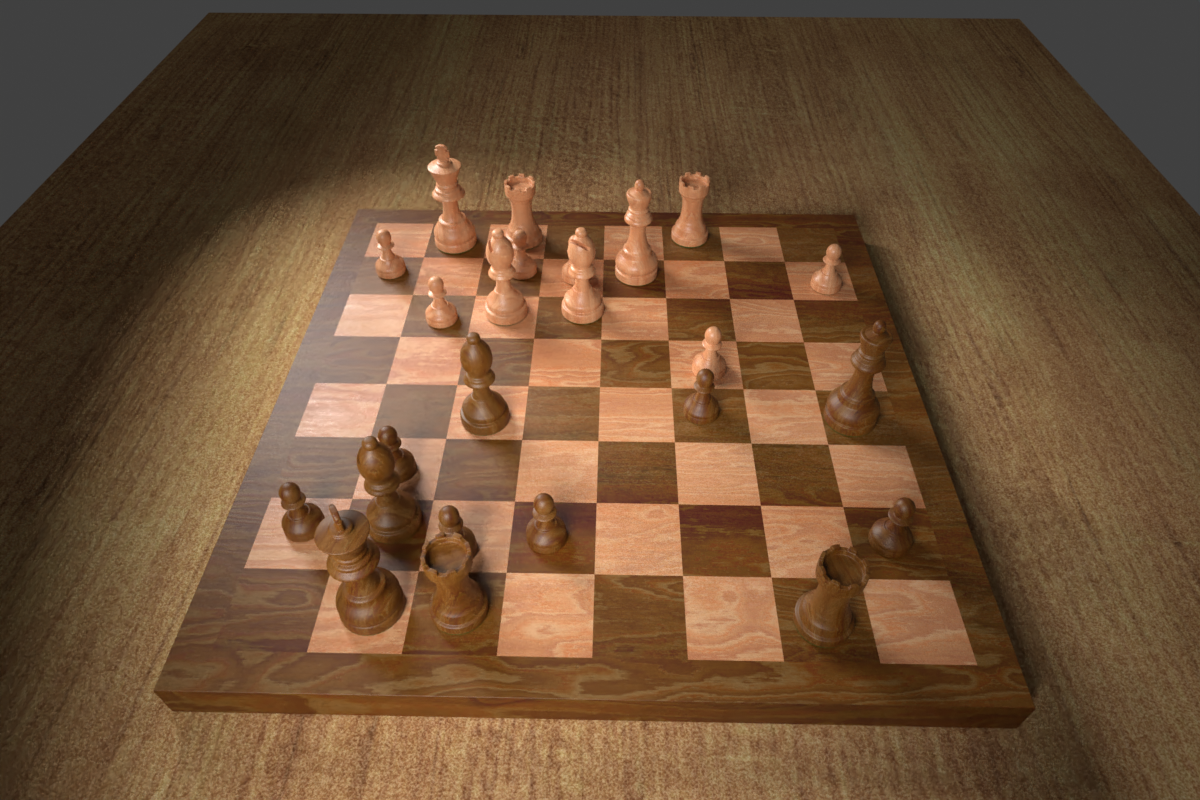
\includegraphics[width=\textwidth]{3828}
        \caption{original}
        \label{fig:occupancy_classification_samples_original}
    \end{subfigure}
    \hfill
    \begin{subfigure}[b]{0.47\textwidth}
        \centering
        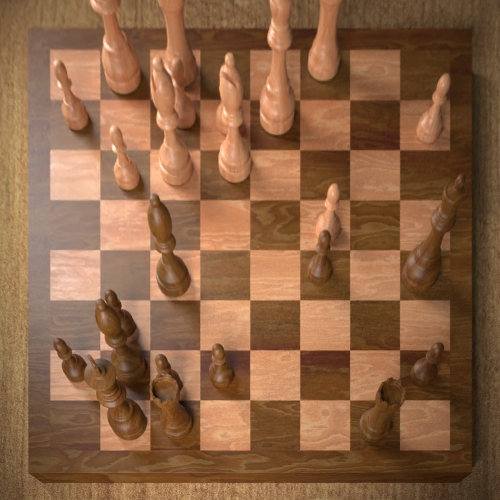
\includegraphics[width=\textwidth]{3828_unwarped}
        \caption{warped}
        \label{fig:occupancy_classification_samples_warped}
    \end{subfigure}
    
    \bigskip
    \begin{subfigure}[b]{0.47\textwidth}
        \centering
        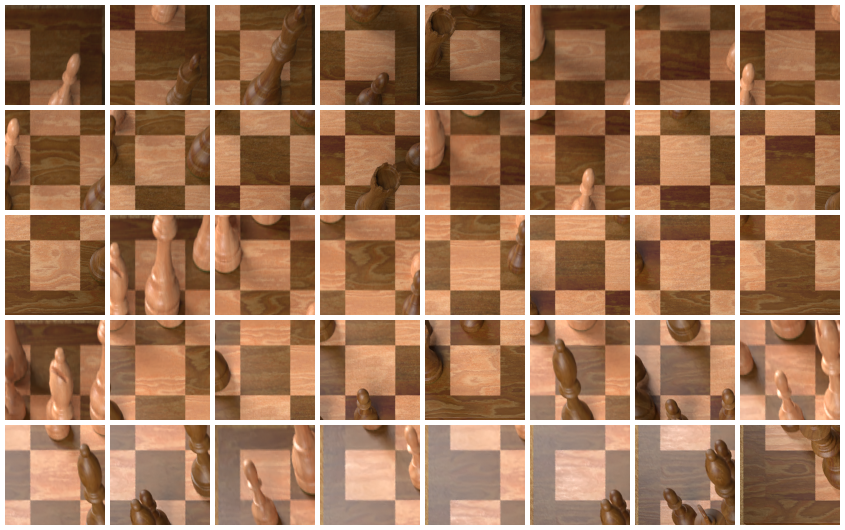
\includegraphics[width=\textwidth]{3828_empty}
        \caption{all 32 empty samples}
        \label{fig:occupancy_classification_samples_empty}
    \end{subfigure}
    \hfill
    \begin{subfigure}[b]{0.47\textwidth}
        \centering
        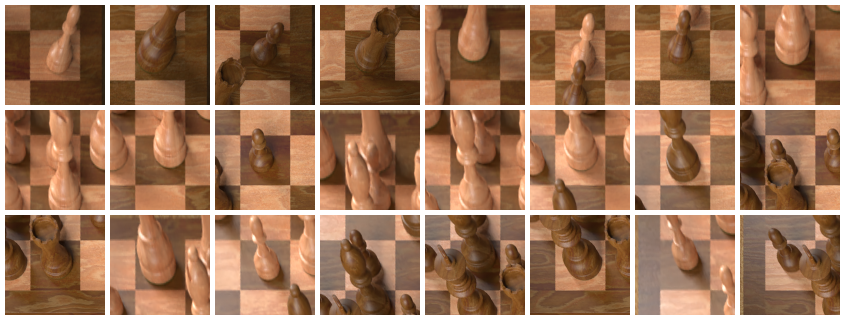
\includegraphics[width=\textwidth]{3828_occupied}
        \caption{all 24 occupied samples}
        \label{fig:occupancy_classification_samples_occupied}
    \end{subfigure}
    \caption[The process of obtaining samples for occupancy classification from a chessboard image.]{The process of obtaining samples for occupancy classification from a chessboard image. First, the original image \subref{fig:occupancy_classification_samples_original} is warped to a two-dimensional overhead view, \subref{fig:occupancy_classification_samples_warped}. Then, all squares are cropped (with a 50\% increase in width and height to include contextual information). Finally, the cropped squares are annoted using the \gls{fen} groundtruth as either empty \subref{fig:occupancy_classification_samples_empty} or occupied \subref{fig:occupancy_classification_samples_occupied}.}
    \label{fig:occupancy_classification_samples}
\end{figure}

Cropping the squares from the warped image is trivial because the squares are of equal size.
In training the occupancy classifiers, it is conjectured that it would be useful to include contextual information with each square; therefore, the squares are not cropped tightly around their boundaries but instead with a 50\% increase in length on all four sides, as shown in \cref{fig:occupancy_classification_samples_empty,fig:occupancy_classification_samples_occupied}.
This might aid the classifier's decision in difficult situations where a chess piece from another square reaches into the cropped one due to the camera perspective.

\subsubsection{\Glspl{cnn}}
Six \gls{cnn} architectures are devised for the occupancy classification task, of which two accept $100\times 100$ pixel input images and the remaining four require the images to be of size $50\times 50$ pixels.
They differ in the number of convolution layers, pooling layers, and fully connected layers.
When referring to these models, we shall use a 4-tuple consisting of the input side length and the three aforementioned criteria.
\Cref{fig:occupancy_convnet} depicts the architecture of the \gls{cnn} $(100, 3, 3, 3)$ model which achieves the greatest validation accuracy of these six models.
\begin{figure}
    \centering
    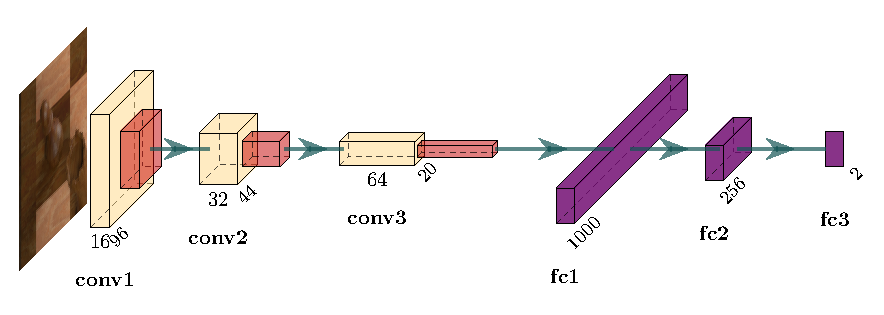
\includegraphics[width=\textwidth]{occupancy_convnet}
    \caption[Architecture of the CNN $(100,3,3,3)$ network for occupancy classification.]{
        Architecture of the \gls{cnn} $(100,3,3,3)$ network for occupancy classification.
        The input is a three-channel \gls{rgb} image with $100\times 100$ pixels.
        There are two convolutional layers (yellow) with a kernal size of $5 \times 5$ and stride $1$, meaning that each convolutional layer reduces the width and height by $4$.
        The final convolutional layer has a kernel size of $3 \times 3$, thus only reducing the input size by two.
        Starting with 16 filters in the first convolutional layer, the number of channels is doubled in each subsequent layer, as is common practice in \glspl{cnn} \cite{simonyan2015}.
        Each convolutional layer uses the \gls{relu} activation function and is followed by a max pooling layer with a $2\times 2$ kernel that is moved with a stride of $2$ such that the width and height are halved.
        Finally, the output of the last pooling layer is reshaped to a 640,000-dimensional vector that passes through two fully connected \gls{relu}-activated layers before reaching the final fully connected layer with softmax activation.
    }
    \label{fig:occupancy_convnet}
\end{figure}
The final fully connected layer in each model contains two output units that represent the two classes (occupied and empty).
The models are trained using the cross-entropy loss function on the outputs.
Training proceeds using the popular \emph{Adam} optimizer \cite{kingma2017} with a learning rate of $0.001$ for three whole passes over the training set using a batch size of 128.
After every 100 steps, the model's loss and accuracy is computed over the entire validation set, the results of which are reported in \cref{fig:occupancy_cnn_loss_accuracy}.
\begin{figure}
    \makebox[\textwidth][c]{
        \begin{subfigure}{.45\textwidth}
            \begin{tikzpicture}
                \begin{axis}[
                    no markers,
                    xlabel={step},
                    ylabel={cross-entropy loss},
                    title={Loss},
                    scale only axis,
                    width=.9\textwidth,
                    legend style={at={(0.98,0.98)},anchor=north east}
                ]
                    \addplot table [x=Step, y=Value, col sep=comma] {data/run-occupancy_classifier_CNN100_3Conv_3Pool_3FC_train-tag-Loss.csv};
                    \addplot table [x=Step, y=Value, col sep=comma] {data/run-occupancy_classifier_CNN100_3Conv_3Pool_3FC_val-tag-Loss.csv};
                    \legend{training,validation}
                \end{axis}
            \end{tikzpicture}
        \end{subfigure}
        \hfill
        \begin{subfigure}{.45\textwidth}
            \begin{tikzpicture}
                \begin{axis}[
                    no markers,
                    xlabel={step},
                    ylabel={accuracy},
                    title={Accuracy},
                    scale only axis,
                    width=.9\textwidth,
                    ylabel near ticks,
                    yticklabel pos=right,
                    legend style={at={(0.98,0.02)},anchor=south east}
                ]
                    \addplot table [x=Step, y=Value, col sep=comma] {data/run-occupancy_classifier_CNN100_3Conv_3Pool_3FC_train-tag-Accuracy.csv};
                    \addplot table [x=Step, y=Value, col sep=comma] {data/run-occupancy_classifier_CNN100_3Conv_3Pool_3FC_val-tag-Accuracy.csv};
                    \legend{training,validation}
                \end{axis}
            \end{tikzpicture}
        \end{subfigure}
    }
    \caption[Loss and accuracy during training on both the training and validation sets for the CNN $(100,3,3,3)$ model.]{Loss and accuracy during training on both the training and validation sets for the \gls{cnn} $(100,3,3,3)$ model. The best validation accuracy is 99.71\%.}
    \label{fig:occupancy_cnn_loss_accuracy}
\end{figure}
The model converges smoothly to a very low loss value, achieving a training accuracy of 99.70\% and validation accuracy of 99.71\%.
Due to the fact that the difference between training and validation accuracy is very small (in fact, the validation accuracy even happens to be slightly above the training accuracy), we conclude that the model does not overfit the training set.

\subsubsection{Transfer learning on deeper models}
VGG \cite{simonyan2015}
ResNet \cite{he2016}
AlexNet \cite{krizhevsky2017}
ImageNet \cite{deng2009}


\todo{todo: explain how this was done and explain tradeoff (significantly more parameters in model)}

\subsubsection{Analysis}
Each model is trained separately on the dataset of squares that are cropped to include contextual information (by increasing the bounding box by 50\% in each direction), and the same samples except that the squares are cropped tightly.
In each case, the model trained on the samples that contained contexual information outperfomed its counterpart trained on tightly cropped samples, confirming the hypothesis that the information around the square itself is useful.


\begin{table}
    \centering
    \makebox[\textwidth][c]{
        \pgfplotstabletypeset[
            col sep=tab,
            columns={context,model,parameters,val_accuracy,val_precision/occupied,val_recall/occupied,val_misclassified,train_accuracy},
            every head row/.style={%
                before row=\toprule,
                after row=\midrule%
            },
            every last row/.style={
                after row=\bottomrule
            },
            columns/model/.style={
                string type
            },
            columns/context/.style={
                string type,
                column name={}
            },
            columns/val_accuracy/.style={
                dec sep align,
                postproc cell content/.append code={
                    \ifnum1=\pgfplotstablepartno
                        \pgfkeysalso{@cell content/.add={}{\%}}%
                    \fi
                },
                fixed,
                fixed zerofill,
                column name={accuracy}
            },
            columns/train_accuracy/.style={
                dec sep align,
                postproc cell content/.append code={
                    \ifnum1=\pgfplotstablepartno
                        \pgfkeysalso{@cell content/.add={}{\%}}%
                    \fi
                },
                fixed,
                fixed zerofill,
                column name={\makecell{training \\ accuracy}}
            },
            columns/val_precision/occupied/.style={
                dec sep align,
                precision=3,
                fixed,
                fixed zerofill,
                column name={precision}
            },
            columns/val_recall/occupied/.style={
                dec sep align,
                precision=3,
                fixed,
                fixed zerofill,
                column name={recall}
            },
            columns/val_misclassified/.style={
                column name={\makecell{errors}}
            },
        ]{data/occupancy_classifier.dat}
    }
    \caption[Performance of all occupancy classification models on the validation set.]{
        Performance of all occupancy classification models on the validation set.
        For the \gls{cnn} models, the 4-tuple denotes the length of the square input size in pixels, the number of convolution layers, the number of pooling layers, and the number of fully connected layers.
        The check mark in the left column indicates whether the input samples contained contextual information (cropped to include part of the adjacent squares).
        In the penultimate column, the total number of misclassifications in the validation set are reported (the validation set consists of 9,346 samples).
        The training accuracy is given in the rightmost column for comparison.
        Notice that there is no significant difference between the validation and training accuracies, indicating that none of the models suffer from overfitting.
    }
\end{table}

\begin{figure}
    \makebox[\textwidth][c]{
        \begin{subfigure}{.45\textwidth}
            \begin{tikzpicture}
                \begin{axis}[
                    no markers,
                    xlabel={step},
                    ylabel={cross-entropy loss},
                    title={Loss},
                    scale only axis,
                    width=.9\textwidth,
                    legend style={at={(0.98,0.98)},anchor=north east}
                ]
                    \addplot table [x=Step, y=Value, col sep=comma] {data/run-occupancy_classifier_ResNet_train-tag-Loss.csv};
                    \addplot table [x=Step, y=Value, col sep=comma] {data/run-occupancy_classifier_ResNet_val-tag-Loss.csv};
                    \legend{training,validation}
                \end{axis}
            \end{tikzpicture}
        \end{subfigure}
        \hfill
        \begin{subfigure}{.45\textwidth}
            \begin{tikzpicture}
                \begin{axis}[
                    no markers,
                    xlabel={step},
                    ylabel={accuracy},
                    title={Accuracy},
                    scale only axis,
                    width=.9\textwidth,
                    ylabel near ticks,
                    yticklabel pos=right,
                    legend style={at={(0.98,0.02)},anchor=south east}
                ]
                    \addplot table [x=Step, y=Value, col sep=comma] {data/run-occupancy_classifier_ResNet_train-tag-Accuracy.csv};
                    \addplot table [x=Step, y=Value, col sep=comma] {data/run-occupancy_classifier_ResNet_val-tag-Accuracy.csv};
                    \legend{training,validation}
                \end{axis}
            \end{tikzpicture}
        \end{subfigure}
    }
    \caption[Loss and accuracy during training on both the training and validation sets for the ResNet model.]{Loss and accuracy during training on both the training and validation sets for the ResNet model. The best validation accuracy is 99.96\%.}
    \label{fig:occupancy_resnet_loss_accuracy}
\end{figure}

\begin{figure}
    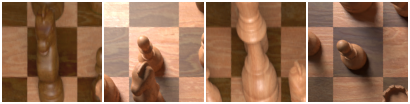
\includegraphics[width=\textwidth]{ResNet_val_mistakes.png}
    \caption[The four samples that the ResNet model misclassified in the validation set.]{The four samples that the ResNet model misclassified in the validation set. The left sample depicts an empty square, and the remaining three are of occupied squares.}
    \label{fig:occupancy_resnet_mistakes}
\end{figure}

\subsection{Piece classification}
Now that the occupancy of each square on the chessboard can be detected to a high degree of accuracy, the next step is to classify the piece in each of the occupied squares.
We require a 12-way classifier that takes as input a cropped image of an occupied square and will output the chess piece on that square. 
There are six types of chess pieces (pawn, knight, bishop, rook, queen, and king), and each piece can either be white or black in colour, thus there are 12 classes of pieces.

We must pay some special attention to how the pieces are cropped. 
Simply following the approach described in \cref{sec:occupancy_classification} for cropping squares does not give enough information to classify pieces.
Especially tall pieces at the back of the board would be cropped in a manner such that only the bottom part of the piece remains in the \gls{roi}. 
Consider for example the white king in \cref{fig:occupancy_classification_samples}.
Cropping only the square it is located in would not include its crown which is an important feature needed to distinguish between kings and queens.
Instead, we must choose a rectangular bounding box that is tall enough to account for the perspective distortion.

The camera perspective causes another phenomenon that we must account for: pieces on the left of the board tend to `slant' to the left, and vice-versa on the right.
This is due to the vanishing point of the normals of the chessboard surface being roughly centred horizontally with regards to the location of the chessboard itself, as illustrated in \cref{fig:occupancy_classification_normals}.
\begin{figure}
    \centering
    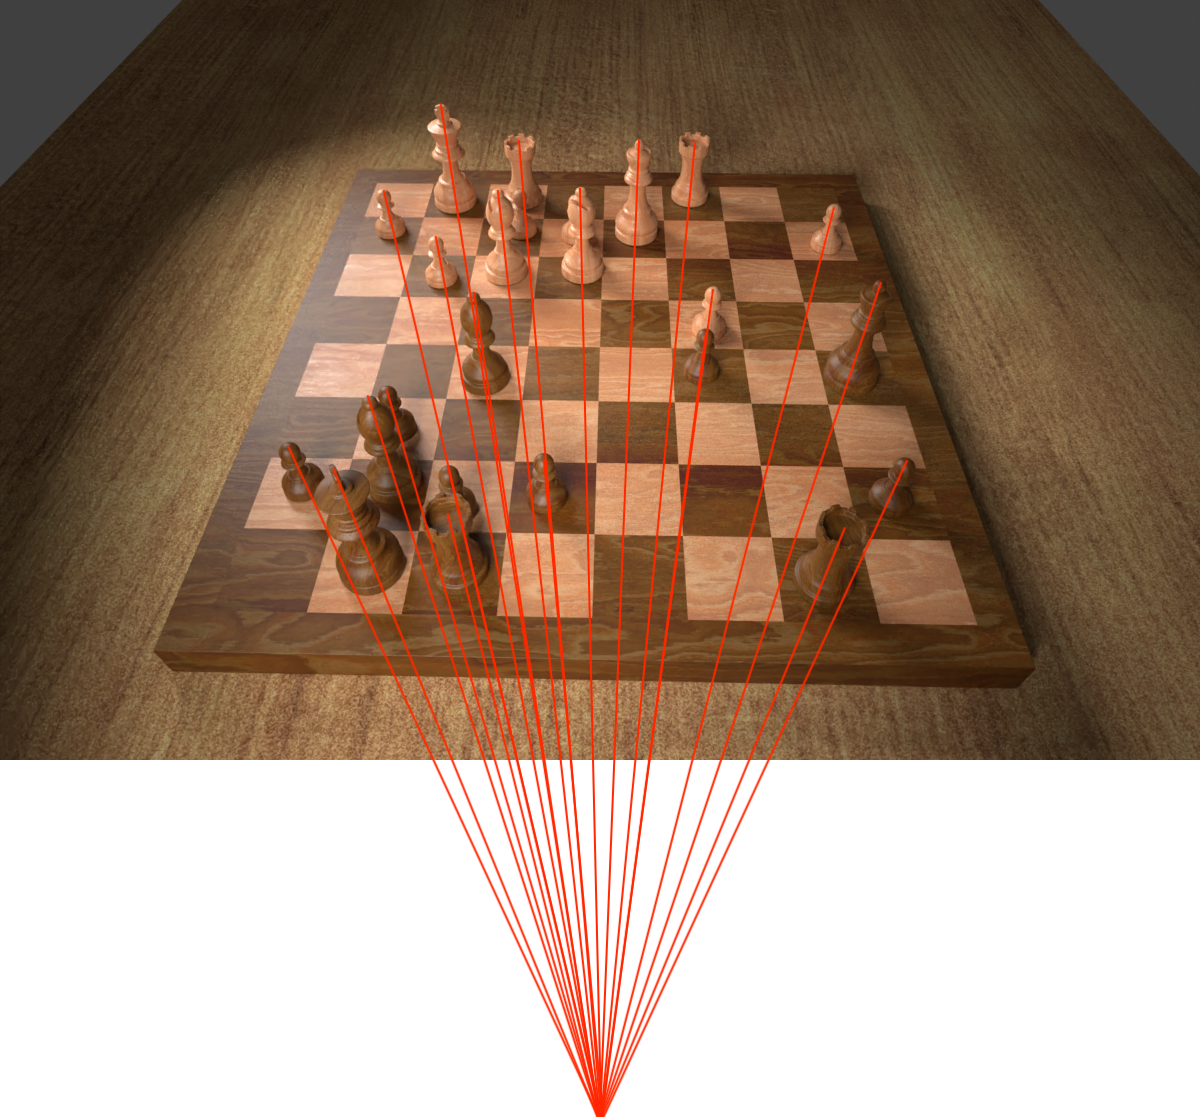
\includegraphics[width=.7\textwidth]{3828_normals.png}
    \caption{The normals converge to a single vanishing point which is below the image. We will assume that the vanishing point is roughly horizontally centred with the chessboard, as this corresponds to how chessboards are usually photographed. As a result, pieces on left `lean' left, and vice-versa on the right.}
    \label{fig:occupancy_classification_normals}
\end{figure}
Hence, we must extend the \gls{roi} horizontally in the appropriate direction.

To obtain the \glspl{roi}, we first warp the input image of the chessboard as described in \cref{sec:occupancy_classification} and exemplified in \cref{fig:occupancy_classification_samples_warped}.

\begin{table}
    \centering
    \makebox[\textwidth][c]{
        \pgfplotstabletypeset[
            col sep=tab,
            columns={model,parameters,val_accuracy,val_misclassified,train_accuracy},
            every head row/.style={%
                before row=\toprule,
                after row=\midrule%
            },
            every last row/.style={
                after row=\bottomrule
            },
            columns/model/.style={
                string type
            },
            columns/val_accuracy/.style={
                dec sep align,
                postproc cell content/.append code={
                    \ifnum1=\pgfplotstablepartno
                        \pgfkeysalso{@cell content/.add={}{\%}}%
                    \fi
                },
                fixed,
                fixed zerofill,
                column name={accuracy}
            },
            columns/train_accuracy/.style={
                dec sep align,
                postproc cell content/.append code={
                    \ifnum1=\pgfplotstablepartno
                        \pgfkeysalso{@cell content/.add={}{\%}}%
                    \fi
                },
                fixed,
                fixed zerofill,
                column name={\makecell{training \\ accuracy}}
            },
            columns/val_misclassified/.style={
                column name={\makecell{errors}}
            },
        ]{data/piece_classifier.dat}
    }
    \caption[Performance of all piece classifiers on the validation set.]{
        Performance of all piece classifiers on the validation set.
    }
\end{table}

\section{An approach based on object detection}
\section{Identifying plausible game states}

\end{document}